\documentclass{article}

\usepackage{icpc_problem} % or wherever this package is stored
\usepackage[english]{babel}
\usepackage[usenames,dvipsnames,svgnames,table]{xcolor}
\usepackage{amssymb}
\usepackage{float}
\usepackage{tikz}
\def\NN{\mathbb{N}}
\def\ZZ{\mathbb{Z}}
\def\prob{\mathbb{P}}
\def\esp{\mathbb{E}}
\def\ag{\mathcal{A}}
\def\CC{\mathcal{C}}


\title{Camino del drag\'on}
\author{Sebasti\'an Barbieri}
\keywords{bd}
\comments{none}
\difficulty{5} % the difficulty should be a non-negative integer

\begin{document}

\begin{problemDescription}

Nuestro h\'eroe Olon-sonk\'u debe recorrer el camino del drag\'on para llegar al planeta de Jorgesama y aumentar su poder de pelea. Desgraciadamente el camino del drag\'on no es una l\'inea recta, sino que es un camino fractal conocido como la curva del drag\'on de Highway.
\begin{center}
	\includegraphics[scale=0.6]{dragon.png}
\end{center}

Si bien nuestro amigo Olon-sonk\'u tiene una gran fuerza f\'isica, su inteligencia no se equipara y tiene problemas para realizar hasta el m\'as simple de los c\'alculos artim\'eticos. Para lograr su cometido debe lograr calcular las coordenadas del planeta del gran Jorgesama lo cual le resulta muy complicado. Por fortuna su amiga Bulnelman planea ayudarlo a realizar esta tarea.

Bulnelman estudia el camino del drag\'on y descubre lo siguiente:

Supongamos que Olon-sonk\'u comienza en la posici\'on $(0,0)$ mirando al norte. El camino del Drag\'on se describe de la siguiente forma: Denoremos por $A$ la acci\'on de avanzar un paso, $R$ rotar $90^{\circ}$ a la derecha y $L$ rotar $90^{\circ}$ a la izquierda. Consideremos el sistema de reescritura siguiente donde cada letra $a,b$ se reemplaza por la cadena de caracteres de la derecha.

$$a \rightarrow aRbAR$$
$$b \rightarrow LAaLb$$

Por ejemplo, si comenzamos con la cadena $Aa$ y aplicamos las reglas dos veces obtendremos:

$$Aa \rightarrow AaRbAR \rightarrow AaRbARRLAaLbAR $$

El camino del drag\'on est\'a determinado por la secuencia de instrucciones obtenidas al repetir las reglas de escritura iterativamente e ignorar las apariciones de $a$ y $b$. Por ejemplo, si consideramos las primeras dos iteraciones y eliminamos las apariciones obtenemos la cadena $ARARRLALAR$. Esto significa que el camino es el siguiente:

\begin{itemize}
	\item Comenzar en (0,0) mirando al norte
	\item Avanzar un paso: Llega a (0,1) y mira al norte.
	\item Rotar a la derecha y avanzar, llega a (1,1) y mira al este.
	\item Rotar dos veces a la derecha y una a la izquierda y avanzar, llega a (1,0) y mira al sur.
	\item Rotar a la izquierda y avanzar, llega a (2,1) y mira al este.
	\item Rota a la derecha, Termina en (2,1) mirando al sur.
\end{itemize}

\begin{figure}[h]
\begin{center}
		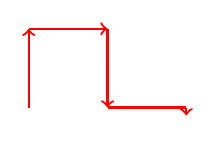
\begin{tikzpicture}
	\draw[thick, red, ->] (0,0) to (0,1);
	\draw[thick, red, ->] (0,1) to (1,1);
	\draw[thick, red, ->] (1,1) to (1,0);
	\draw[thick, red, -] (1,0) to (2,0);
	\draw[thick, red, ->] (2,0) to (2,-0.1);
	\end{tikzpicture}
\end{center}
	\caption{Primeros pasos del camino del drag\'on}
\end{figure}


Digamos que el camino tiene largo $n$ si se ejecuta la acci\'on avanzar $n$ veces. Supongamos que Bulnelman sabe que la casa de el gran Jorgesama se encuentra luego de recorrer $n$ pasos. ?`Puedes ayudarnos a saber cual es la posici\'on exacta de la casa del gran Jorgesama?

.\end{problemDescription}

\begin{inputDescription}
El input consiste en una l\'inea que contiene un entero positivo $n$ describiendo el largo del camino del drag\'on
\end{inputDescription}

\begin{outputDescription}
El output consiste en una l\'inea que contiene dos enteros $x$ e $y$ determinando las coordenadas de la casa del gran Jorgesama.
\end{outputDescription}

\begin{sampleInput}
5
15
10000
10000000000000
\end{sampleInput}
\begin{sampleOutput}
TODO
\end{sampleOutput}

\begin{scoreDescription}
\score{10} Se probar\'an varios casos en donde $1 \leq n \leq 10$.
\score{20} Se probar\'an varios casos en donde $1 \leq n \leq 100$.
\score{40} Se probar\'an varios casos en donde $1 \leq n \leq 10^5$.
\score{30} Se probar\'an varios casos donde $1 \leq n \leq 10^{12}$. 
\end{scoreDescription}

\end{document}


